\documentclass{beamer}
\usetheme{Warsaw}
\definecolor{RHUL-light}{HTML}{eb641e}
\definecolor{RHUL-dark}{HTML}{202a30}
\setbeamercolor{structure}{fg=RHUL-light!90!RHUL-dark}
\usepackage{tikz}
\usepackage{subcaption}
\usetikzlibrary{positioning,arrows, automata}


% syntax highlighting
\newcommand{\mvar}[1]{$\;\texttt{\textcolor{black}{#1}}\;$}
\newcommand{\mkey}[1]{$\;\texttt{\textcolor{orange}{#1}}\;$}
\newcommand{\mmod}[1]{$\;\texttt{\textcolor{purple}{#1}}\;$}
\newcommand{\mdef}[1]{$\;\texttt{\textcolor{blue}{#1}}\;$}
\newcommand{\mcon}[1]{$\;\texttt{\textcolor{brickred}{#1}}\;$}
\newcommand{\mtype}[1]{$\;\texttt{\textcolor{brown}{#1}}\;$}
\newcommand{\mpar}[1]{$(#1)$}
\newcommand{\mnil}[1]{\mcon{[]}}
\newcommand{\cons}[3]{\mpar{\mval{#1}\mcon{#2}\mval{#3}}}
\newcommand{\ra}[0]{$\;\rightarrow\;$}
\newcommand{\Ra}[0]{$\;\Rightarrow\;$}
\newcommand{\ind}[0]{$\;\;\;\;$}

\newcommand{\plusplus}{\mathbin{+\!\!\!+}}

%\setlength\abovedisplayskip{4pt}
%\setlength\abovecaptionskip{0pt}
%\setlength\belowdisplayskip{0pt}
%\setlength\belowcaptionskip{0pt}
%\setlength\intextsep{4pt}

% grammars
\newcommand{\nt}[1]{\texttt{#1}}
\newcommand{\pr}[1]{\textit{\texttt{#1}}}
\newcommand{\tm}[1]{\underline{#1}}
\newcommand{\lf}[1]{\texttt{#1}.}
\newcommand{\rf}[1]{@\texttt{#1}.}
\newcommand{\f}[1]{@\texttt{#1}}
\newcommand{\ff}[1]{\texttt{#1}}

\newcommand{\app}[1]{\textsc{#1}}

% sets
\newcommand{\set}[2]{\{\;#1\;\;|\;\;#2\;\}}
\newcommand{\sand}[0]{,\;}

% quantification
\newcommand{\univ}[2]{\forall(#1)\;(#2)}
\newcommand{\exis}[2]{\exists(#1)\;(#2)}

% administration
\newcommand{\toindex}[1]{\emph{#1}\index{#1}}
\newcommand{\toindexwith}[2]{\emph{#1}\index{#2}}

% visit-sequences
\newcommand{\vsrelsize}{1.5cm}
\tikzstyle{vsstyle}=[shape=rectangle,draw]

\newcommand{\myvs}[3]{
\draw[style=vsstyle] (#1 *\vsrelsize,0) rectangle (#2 *\vsrelsize, 0.9cm) node[anchor=north east] (v1#1) {\begin{varwidth}{\vsrelsize}\small{#3}\end{varwidth}};
}


% agpictures
\definecolor{light-gray}{gray}{0.83}
\newdimen\agrelsize
\setlength{\agrelsize}{0.30cm}
\tikzstyle{agnontermstyle}=[shape=circle,draw,minimum size=\agrelsize]
\tikzstyle{agchldstyle}=[shape=circle,fill=red!70,minimum size=\agrelsize]
\tikzstyle{agattrstyle}=[shape=rectangle,draw,minimum size=\agrelsize,]
\tikzstyle{agdepstyle}=[black,>=triangle 60]
\tikzstyle{agidpstyle}=[gray,>=triangle 60]
\tikzstyle{inputstyle}=[shape=rectangle,fill=light-gray,draw,minimum size=\agrelsize]
\tikzstyle{outputstyle}=[shape=rectangle,draw,minimum size=\agrelsize]
\newcommand{\agcoordpary}{6}   %% y-coordinate of parent attributes
\newcommand{\agcoordchldy}{0}  %% y-coordinate of child attributes
\newcommand{\agcoordlocy}{3}   %% y-coordinate of local attributes
\newcommand{\agbeginprod}[5]{} %% you could begin a picture here
\newcommand{\agendprod}[5]{}   %% you could end a picture here
\newcommand{\agparent}[5]{ \draw (#4 \agrelsize,\agcoordpary \agrelsize) node [style=agnontermstyle] (#3) {}; \draw (#3.north) node [anchor=south] {\footnotesize{ #2 }}; \draw (#3.south) node [anchor=north] {\footnotesize{ #5 }}; }
\newcommand{\agparattr}[6]{ \draw (#4 \agrelsize,\agcoordpary \agrelsize) node [style=#6] (#3) {}; \draw (#3.south) node [anchor=south] {\tiny{#2}}; }
\newcommand{\agchldattr}[6]{ \draw (#4 \agrelsize,\agcoordchldy \agrelsize) node [style=#6] (#3) {}; \draw (#3.north) node [anchor=north] {\tiny{#2}}; }
\newcommand{\agchldnonterm}[5]{ \draw (#4 \agrelsize,\agcoordchldy \agrelsize) node [style=agnontermstyle] (#3) {}; \draw (#3.south) node [anchor=north] {\footnotesize{ #2:#5 }}; }
\newcommand{\agchldterm}[5]{ \draw (#4 \agrelsize,\agcoordchldy \agrelsize) node [style=agchldstyle] (#3) {}; \draw (#3.south) node [anchor=north] {\footnotesize{ #2 }}; }
\newcommand{\agsibline}[3]{ \draw (#2.east) -- (#3.west); }
\newcommand{\agdeplineupdown}[4]{ \draw[->,style=agdepstyle] (#2.north) .. controls +(0,1) and +(0,-1) .. (#3.south); }
\newcommand{\agdeplineupup}[5]{ \draw[->,style=agdepstyle] (#2.north) .. controls +(0,#5) and +(0,#5) .. (#3.north); }
\newcommand{\agidplineup}[5]{ \draw[->,style=agidpstyle] (#2.north) .. controls +(0,#5) and +(0,#5) .. (#3.north); }
\newcommand{\agidplineupdown}[5]{ \draw[->,style=agidpstyle] (#2.north) .. controls +(0,#5) and +(0,-#5) .. (#3.south); }
\newcommand{\agdeplineupupbold}[4]{ \draw[->,style=agdepstyle,line width=2pt] (#2.north) .. controls +(0,1) and +(0,1) .. (#3.north); }
\newcommand{\agdeplinedowndown}[5]{ \draw[->,style=agdepstyle] (#2.south) .. controls +(0,-#5) and +(0,-#5) .. (#3.south); }
\newcommand{\agidplinedown}[5]{ \draw[->,style=agidpstyle] (#2.south) .. controls +(0,-#5) and +(0,-#5) .. (#3.south); }
\newcommand{\agdeplinedowndownbold}[4]{ \draw[->,style=agdepstyle,line width=2pt] (#2.south) .. controls +(0,-1) and +(0,-1) .. (#3.south); }
\newcommand{\agdeplinedowndowndashed}[5]{ \draw[->,style=agidpstyle, dashed] (#2.south) .. controls +(0,-#5) and +(0,-#5) .. (#3.south); }
\newcommand{\agdeplinedownup}[4]{ \draw[->,style=agdepstyle] (#2.south) .. controls +(0,-1) and +(0,1) .. (#3.north); }
\newcommand{\agpicture}[1]{ \begin{tikzpicture}\input{#1.tikz}\end{tikzpicture} }

\newcommand{\mypic}[2]{
 \begin{figure}[ht]
  \centering
    \agpicture{diagrams/#1}
    \caption{#2}
  \label{fig:#1}
 \end{figure}
}

\newcommand{\mypicstar}[2]{
 \begin{figure*}[t]
  \centering
    \agpicture{diagrams/#1}
    \caption{#2}
  \label{fig:#1}
 \end{figure*}
}

\newcommand{\mydoublepic}[6]{
 \begin{figure*}[t]
  \centering
    \begin{minipage}[a]{#3\textwidth}
        \agpicture{diagrams/#2}
    \end{minipage}
    \begin{minipage}[a]{#5\textwidth}
        \agpicture{diagrams/#4}
    \end{minipage}
    \caption{#6}
  \label{fig:#1}
 \end{figure*}
}

\newcounter{algoctr}
\setcounter{algoctr}{-1}
\newcounter{cfctr}
\setcounter{cfctr}{-1}
\newcounter{defctr}



\title{Linearly Ordered Attribute Grammar scheduling using SAT-solving}
\author[shortname]{Jeroen Bransen \inst{1} \and 
                  \underline{L. Thomas van Binsbergen} \inst{2} \and\\ 
                   Atze Dijkstra \inst{1} \and 
                    Koen Claessen \inst{3}}
\institute[shortinst]{
    \inst{1} Utrecht University \and
    \inst{2} Royal Holloway, University of London \and
    \inst{3} Chalmers University of Technology}
\date {TACAS 2015, ETAPS, London}

\begin{document}

\begin{frame}
    \maketitle
\end{frame}

\begin{frame}
    \frametitle{Attribute Grammars}
    \begin{itemize}
        \item Attribute Grammars describe computations over trees.
        \item Useful in compiler construction, e.g. for:\\
                Code generation, static analysis, semantic evaluation.
        \item An AG compiler generates an evaluator from a description.
        \item To generate a \emph{strict} evaluator scheduling is required.
        \item This scheduling problem is NP-hard.
    \end{itemize}
\end{frame}

\begin{frame}
    \frametitle{Compile-time scheduling}
    \begin{itemize}
        \item No compile-time scheduling: 
            \begin{itemize}
                \item Generate lazy code.
            \end{itemize}
        \item Some compile-time scheduling: 
            \begin{itemize}
                \item Find multiple schedules, covering all possible trees.
                \item The actual schedule depends on the input tree.
                \item Absolutely Non-Circular Attribute Grammars (ANCAGs).
                \item Kennedy-Warren algorithm.
            \end{itemize}
        \item Full compile-time scheduling:
            \begin{itemize}
                \item Find a single evaluation order.
                \item It needs to be compatible with all possible trees.
                \item Linearly Ordered Attribute Grammars (LOAGs).
                \item Kastens' algorithm (schedules subclass OAG).
            \end{itemize}
    \end{itemize}
\end{frame}

\begin{frame}
    \frametitle{Motivation}
    \begin{itemize}
        \item Many tools at Utrecht University are developed using AGs.
        \item Large projects require efficient and strict code.
        \item Main motivation is the Utrecht Haskell Compiler.         
    \end{itemize}
\end{frame}

\begin{frame}
    \frametitle{Scheduling the Utrecht Haskell Compiler (UHC)}
    \begin{itemize}
        \item UHC is partly generated from of a large number of AGs.
        \item The ``main AG'' is large indeed:
         \begin{itemize}
            \item 30 non-terminals
            \item 134 productions
            \item 1332 attributes (44.4 per non-terminal!)
            \item 9766 dependencies
         \end{itemize} 
        \item Kastens' algorithm does not find a static evaluation order for the main AG.
        \item We know at least one exists, as Kastens' algorithm can be `helped' to find one
                using 24 \emph{augmenting dependencies}.
    \end{itemize}
\end{frame}

\begin{frame}
    \frametitle{Overview}
    \begin{itemize}
        \item LOAG scheduling problem.
        \item SAT formulation.
        \item Constraint generation using chordal graphs.
    \end{itemize}
\end{frame}

\section{LOAG scheduling problem}
\begin{frame}
    \frametitle{AG descriptions}
    \begin{itemize}
        \item An AG descriptions contains three components:
        \begin{enumerate}
            \item A context-free grammar (describing all possible input trees).
            \item A set of attribute declarations (for every non-terminal).
            \item A definition for every attribute (in each context it appears).
        \end{enumerate}
        \item From the AG description, the AG compiler obtains:
        \begin{enumerate}
            \item A dependency graph for every:
                \begin{itemize} 
                    \item Non-terminal
                    \item Production
                \end{itemize}
        \end{enumerate}
    \end{itemize}
\end{frame}

\begin{frame}
    \frametitle{Non-terminal dependency graphs}
    \begin{itemize}
        \item The non-terminal dependency graph for $X$ contains:
            \begin{itemize}
                \item The non-terminal $X$ 
                \item All attributes of $X$ as vertices.
            \end{itemize}
    \end{itemize}
    \begin{figure}
        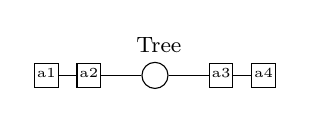
\begin{tikzpicture}

\agbeginprod{0}{Tree}{lhs}{Tree}{10.2} %
\agparent{0}{Tree}{lhs}{5.1}{} %
\agparattr{0}{a1}{lhsIlab}{0.5}{Int}{outputstyle} %
\agparattr{0}{a2}{lhsIvals}{2.3}{[Int]}{outputstyle} %
\agparattr{0}{a3}{lhsSlab}{7.8999999999999995}{Int}{outputstyle} %
\agparattr{0}{a4}{lhsSvals}{9.7}{[Int]}{outputstyle} %
\agsibline{0}{lhsIlab}{lhsIvals} %
\agsibline{0}{lhsIvals}{lhs} %
\agsibline{0}{lhs}{lhsSlab} %
\agsibline{0}{lhsSlab}{lhsSvals} %
        \end{tikzpicture}
    \caption{Non-terminal Tree for representing binary trees.}
    \end{figure}
\end{frame}

\begin{frame}
    \frametitle{Production dependency graph}
    \begin{itemize}
        \only<1,2>{
        \item A production graph contains:
            \begin{itemize} 
                \item A parent node for the production's left-hand side ($\mathit{lhs}$). 
                \item Children for all non-terminal occurrences of the right-hand side.
                \item All attributes of the occurring non-terminals as vertices.
            \end{itemize}
        \item The children are named by the programmer ($l$ and $r$ for Bin).
        \item The vertices are also called \emph{attribute occurrences}. 
        }
    \end{itemize}
    \only<2>{
    \begin{figure}
        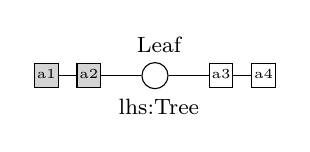
\begin{tikzpicture}
\agbeginprod{0}{Leaf}{lhs}{Tree}{10.2} %
\agparent{0}{Leaf}{lhs}{5.1}{lhs:Tree} %
\agparattr{0}{a1}{lhsIlab}{0.5}{Int}{inputstyle} %
\agparattr{0}{a2}{lhsIvals}{2.3}{[Int]}{inputstyle} %
\agparattr{0}{a3}{lhsSlab}{7.8999999999999995}{Int}{outputstyle} %
\agparattr{0}{a4}{lhsSvals}{9.7}{[Int]}{outputstyle} %
\agsibline{0}{lhsIlab}{lhsIvals} %
\agsibline{0}{lhsIvals}{lhs} %
\agsibline{0}{lhs}{lhsSlab} %
\agsibline{0}{lhsSlab}{lhsSvals} %
\agendprod{0}{Leaf}{lhs}{Tree}{10.2} %
            \end{tikzpicture}
    \end{figure}
    }
    \only<1>{
    \begin{figure}
        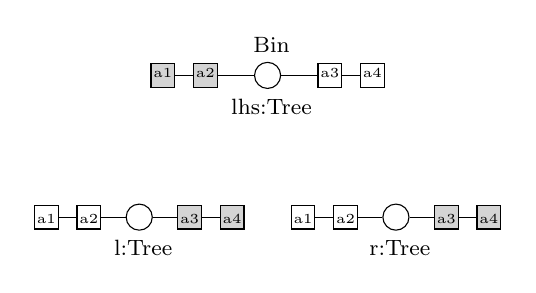
\begin{tikzpicture}
\agbeginprod{0}{Bin}{lhs}{Tree}{19.733333333333334} %
\agparent{0}{Bin}{lhs}{9.866666666666667}{lhs:Tree} %
\agparattr{0}{a1}{lhsIlab}{5.433333333333334}{Int}{inputstyle} %
\agparattr{0}{a2}{lhsIvals}{7.233333333333333}{[Int]}{inputstyle} %
\agparattr{0}{a3}{lhsSlab}{12.5}{Int}{outputstyle} %
\agparattr{0}{a4}{lhsSvals}{14.3}{[Int]}{outputstyle} %
\agchldnonterm{0}{l}{l}{4.433333333333334}{Tree} %
\agchldattr{0}{a1}{lIlab}{0.5}{Int}{outputstyle} %
\agchldattr{0}{a2}{lIvals}{2.3}{[Int]}{outputstyle} %
\agchldattr{0}{a3}{lSlab}{6.566666666666667}{Int}{inputstyle} %
\agchldattr{0}{a4}{lSvals}{8.366666666666667}{[Int]}{inputstyle} %
\agsibline{0}{lIlab}{lIvals} %
\agsibline{0}{lIvals}{l} %
\agsibline{0}{l}{lSlab} %
\agsibline{0}{lSlab}{lSvals} %
\agchldnonterm{0}{r}{r}{15.3}{Tree} %
\agchldattr{0}{a1}{rIlab}{11.366666666666667}{Int}{outputstyle} %
\agchldattr{0}{a2}{rIvals}{13.166666666666668}{[Int]}{outputstyle} %
\agchldattr{0}{a3}{rSlab}{17.433333333333334}{Int}{inputstyle} %
\agchldattr{0}{a4}{rSvals}{19.233333333333334}{[Int]}{inputstyle} %
\agsibline{0}{rIlab}{rIvals} %
\agsibline{0}{rIvals}{r} %
\agsibline{0}{r}{rSlab} %
\agsibline{0}{rSlab}{rSvals} %
\agsibline{0}{lhsIlab}{lhsIvals} %
\agsibline{0}{lhsIvals}{lhs} %
\agsibline{0}{lhs}{lhsSlab} %
\agsibline{0}{lhsSlab}{lhsSvals} %
\agendprod{0}{Bin}{lhs}{Tree}{19.733333333333334} %
        \end{tikzpicture}
    \end{figure}
    }
\end{frame}

\begin{frame}
    \frametitle{Direct dependencies}
    \begin{itemize}
        \item From the AG description \emph{direct dependencies} are obtained.
        \item If attribute $a$ is used in the definition of $b$, then $a\rightarrow b$.
    \end{itemize}
    \begin{figure}
        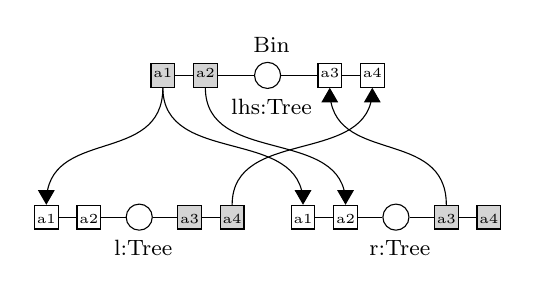
\begin{tikzpicture}
\agbeginprod{0}{Bin}{lhs}{Tree}{19.733333333333334} %
\agparent{0}{Bin}{lhs}{9.866666666666667}{lhs:Tree} %
\agparattr{0}{a1}{lhsIlab}{5.433333333333334}{Int}{inputstyle} %
\agparattr{0}{a2}{lhsIvals}{7.233333333333333}{[Int]}{inputstyle} %
\agparattr{0}{a3}{lhsSlab}{12.5}{Int}{outputstyle} %
\agparattr{0}{a4}{lhsSvals}{14.3}{[Int]}{outputstyle} %
\agchldnonterm{0}{l}{l}{4.433333333333334}{Tree} %
\agchldattr{0}{a1}{lIlab}{0.5}{Int}{outputstyle} %
\agchldattr{0}{a2}{lIvals}{2.3}{[Int]}{outputstyle} %
\agchldattr{0}{a3}{lSlab}{6.566666666666667}{Int}{inputstyle} %
\agchldattr{0}{a4}{lSvals}{8.366666666666667}{[Int]}{inputstyle} %
\agsibline{0}{lIlab}{lIvals} %
\agsibline{0}{lIvals}{l} %
\agsibline{0}{l}{lSlab} %
\agsibline{0}{lSlab}{lSvals} %
\agchldnonterm{0}{r}{r}{15.3}{Tree} %
\agchldattr{0}{a1}{rIlab}{11.366666666666667}{Int}{outputstyle} %
\agchldattr{0}{a2}{rIvals}{13.166666666666668}{[Int]}{outputstyle} %
\agchldattr{0}{a3}{rSlab}{17.433333333333334}{Int}{inputstyle} %
\agchldattr{0}{a4}{rSvals}{19.233333333333334}{[Int]}{inputstyle} %
\agsibline{0}{rIlab}{rIvals} %
\agsibline{0}{rIvals}{r} %
\agsibline{0}{r}{rSlab} %
\agsibline{0}{rSlab}{rSvals} %
\agsibline{0}{lhsIlab}{lhsIvals} %
\agsibline{0}{lhsIvals}{lhs} %
\agsibline{0}{lhs}{lhsSlab} %
\agsibline{0}{lhsSlab}{lhsSvals} %
\agdeplinedownup{0}{lhsIlab}{lIlab}{horunknown} %
\agdeplinedownup{0}{lhsIlab}{rIlab}{horunknown} %
\agdeplinedownup{0}{lhsIvals}{rIvals}{horunknown} %
\agdeplineupupctrl{0}{lSlab}{rIlab}{horleftright}{0.7} %
\agdeplineupupctrl{0}{rSvals}{lIvals}{horrightleft}{0.8} %
\agdeplineupdown{0}{rSlab}{lhsSlab}{horunknown} %
\agdeplineupdown{0}{lSvals}{lhsSvals}{horunknown} %
\agendprod{0}{Bin}{lhs}{Tree}{19.733333333333334} %    
        \end{tikzpicture}
    \end{figure}
\end{frame}


\begin{frame}
    \frametitle{LOAG scheduling}
    \only<1-3>{
    \begin{itemize}
        \item Find a linear order for every production graph, such that:
            \begin{itemize}
                \only<1>{\item[1)] The direct dependencies are `respected'.}
                \only<2,3>{\item[2)] The relative ordering for all occurrences of the same non-terminal are equal.}
                \only<2,3>{\item[] For example, $a3 < a2$ at $r$ $\Rightarrow$ $a3 < a2$ at $l$ and $\mathit{lhs}$, \\ but also at occurrences of Tree in other production graphs.}
            \end{itemize}
    \end{itemize}
    }
    \only<4-5>{
    \begin{figure}
        \begin{tikzpicture}
\agbeginprod{0}{Leaf}{lhs}{Tree}{10.2} %
\agparent{0}{Leaf}{lhs}{5.1}{lhs:Tree} %
\agparattr{0}{a1}{lhsIlab}{0.5}{Int}{inputstyle} %
\agparattr{0}{a2}{lhsIvals}{2.3}{[Int]}{inputstyle} %
\agparattr{0}{a3}{lhsSlab}{7.8999999999999995}{Int}{outputstyle} %
\agparattr{0}{a4}{lhsSvals}{9.7}{[Int]}{outputstyle} %
\agsibline{0}{lhsIlab}{lhsIvals} %
\agsibline{0}{lhsIvals}{lhs} %
\agsibline{0}{lhs}{lhsSlab} %
\agsibline{0}{lhsSlab}{lhsSvals} %
\agdeplinedowndown{0}{lhsIlab}{lhsSlab}{horunknown} %
\agdeplinedowndown{0}{lhsIvals}{lhsSvals}{horunknown} %
\agendprod{0}{Leaf}{lhs}{Tree}{10.2} %            
        \only<4>{
        \node[above=0mm of lhsIlab] {\scriptsize{\textcolor{red}{1}}};
        \node[above=0mm of lhsIvals] {\scriptsize{\textcolor{red}{2}}};
        \node[above=0mm of lhsSlab] {\scriptsize{\textcolor{red}{3}}};
        \node[above=0mm of lhsSvals] {\scriptsize{\textcolor{red}{4}}};
        }
        \only<5>{
        \node[above=0mm of lhsIlab] {\scriptsize{\textcolor{blue}{1}}};
        \node[above=0mm of lhsIvals] {\scriptsize{\textcolor{blue}{3}}};
        \node[above=0mm of lhsSlab] {\scriptsize{\textcolor{blue}{2}}};
        \node[above=0mm of lhsSvals] {\scriptsize{\textcolor{blue}{4}}};
        }
        \end{tikzpicture}
    \end{figure}
    }
    \begin{figure}
        \begin{tikzpicture}
\agbeginprod{0}{Bin}{lhs}{Tree}{19.733333333333334} %
\agparent{0}{Bin}{lhs}{9.866666666666667}{lhs:Tree} %
\agparattr{0}{a1}{lhsIlab}{5.433333333333334}{Int}{inputstyle} %
\agparattr{0}{a2}{lhsIvals}{7.233333333333333}{[Int]}{inputstyle} %
\agparattr{0}{a3}{lhsSlab}{12.5}{Int}{outputstyle} %
\agparattr{0}{a4}{lhsSvals}{14.3}{[Int]}{outputstyle} %
\agchldnonterm{0}{l}{l}{4.433333333333334}{Tree} %
\agchldattr{0}{a1}{lIlab}{0.5}{Int}{outputstyle} %
\agchldattr{0}{a2}{lIvals}{2.3}{[Int]}{outputstyle} %
\agchldattr{0}{a3}{lSlab}{6.566666666666667}{Int}{inputstyle} %
\agchldattr{0}{a4}{lSvals}{8.366666666666667}{[Int]}{inputstyle} %
\agsibline{0}{lIlab}{lIvals} %
\agsibline{0}{lIvals}{l} %
\agsibline{0}{l}{lSlab} %
\agsibline{0}{lSlab}{lSvals} %
\agchldnonterm{0}{r}{r}{15.3}{Tree} %
\agchldattr{0}{a1}{rIlab}{11.366666666666667}{Int}{outputstyle} %
\agchldattr{0}{a2}{rIvals}{13.166666666666668}{[Int]}{outputstyle} %
\agchldattr{0}{a3}{rSlab}{17.433333333333334}{Int}{inputstyle} %
\agchldattr{0}{a4}{rSvals}{19.233333333333334}{[Int]}{inputstyle} %
\agsibline{0}{rIlab}{rIvals} %
\agsibline{0}{rIvals}{r} %
\agsibline{0}{r}{rSlab} %
\agsibline{0}{rSlab}{rSvals} %
\agsibline{0}{lhsIlab}{lhsIvals} %
\agsibline{0}{lhsIvals}{lhs} %
\agsibline{0}{lhs}{lhsSlab} %
\agsibline{0}{lhsSlab}{lhsSvals} %
\agdeplinedownup{0}{lhsIlab}{lIlab}{horunknown} %
\agdeplinedownup{0}{lhsIlab}{rIlab}{horunknown} %
\agdeplinedownup{0}{lhsIvals}{rIvals}{horunknown} %
\agdeplineupupctrl{0}{lSlab}{rIlab}{horleftright}{0.7} %
\agdeplineupupctrl{0}{rSvals}{lIvals}{horrightleft}{0.8} %
\agdeplineupdown{0}{rSlab}{lhsSlab}{horunknown} %
\agdeplineupdown{0}{lSvals}{lhsSvals}{horunknown} %
\agendprod{0}{Bin}{lhs}{Tree}{19.733333333333334} %    

        \only<1>{
        \node[above=0mm of lhsIlab] {\scriptsize{\textcolor{red}{1}}};
        \node[above=0mm of lhsIvals] {\scriptsize{\textcolor{red}{2}}};
        \node[below=0mm of lIlab] {\scriptsize{\textcolor{red}{3}}};
        \node[below=0mm of lIvals] {\scriptsize{\textcolor{red}{4}}};
        \node[below=0mm of lSlab] {\scriptsize{\textcolor{red}{5}}};
        \node[below=0mm of lSvals] {\scriptsize{\textcolor{red}{6}}};
        \node[below=0mm of rIlab] {\scriptsize{\textcolor{red}{7}}};
        \node[below=0mm of rIvals] {\scriptsize{\textcolor{red}{8}}};
        \node[below=0mm of rSlab] {\scriptsize{\textcolor{red}{9}}};
        \node[below=0mm of rSvals] {\scriptsize{\textcolor{red}{10}}};
        \node[above=0mm of lhsSlab] {\scriptsize{\textcolor{red}{11}}};
        \node[above=0mm of lhsSvals] {\scriptsize{\textcolor{red}{12}}};
        }
        \only<2>{
        \node[above=0mm of lhsIlab] {\scriptsize{\textcolor{red}{1}}};
        \node[above=0mm of lhsIvals] {\scriptsize{\textcolor{red}{2}}};
        \node[below=0mm of lIlab] {\scriptsize{\textcolor{red}{3}}};
        \node[below=0mm of lIvals] {\scriptsize{\textcolor{red}{9}}};
        \node[below=0mm of lSlab] {\scriptsize{\textcolor{red}{4}}};
        \node[below=0mm of lSvals] {\scriptsize{\textcolor{red}{10}}};
        \node[below=0mm of rIlab] {\scriptsize{\textcolor{red}{5}}};
        \node[below=0mm of rIvals] {\scriptsize{\textcolor{red}{7}}};
        \node[below=0mm of rSlab] {\scriptsize{\textcolor{red}{6}}};
        \node[below=0mm of rSvals] {\scriptsize{\textcolor{red}{8}}};
        \node[above=0mm of lhsSlab] {\scriptsize{\textcolor{red}{11}}};
        \node[above=0mm of lhsSvals] {\scriptsize{\textcolor{red}{12}}};
        }
        \only<3-5>{
        \node[above=0mm of lhsIlab] {\scriptsize{\textcolor{blue}{1}}};
        \node[above=0mm of lhsIvals] {\scriptsize{\textcolor{blue}{7}}};
        \node[below=0mm of lIlab] {\scriptsize{\textcolor{blue}{2}}};
        \node[below=0mm of lIvals] {\scriptsize{\textcolor{blue}{10}}};
        \node[below=0mm of lSlab] {\scriptsize{\textcolor{blue}{3}}};
        \node[below=0mm of lSvals] {\scriptsize{\textcolor{blue}{11}}};
        \node[below=0mm of rIlab] {\scriptsize{\textcolor{blue}{4}}};
        \node[below=0mm of rIvals] {\scriptsize{\textcolor{blue}{8}}};
        \node[below=0mm of rSlab] {\scriptsize{\textcolor{blue}{5}}};
        \node[below=0mm of rSvals] {\scriptsize{\textcolor{blue}{9}}};
        \node[above=0mm of lhsSlab] {\scriptsize{\textcolor{blue}{6}}};
        \node[above=0mm of lhsSvals] {\scriptsize{\textcolor{blue}{12}}};
        }
         \end{tikzpicture}
        \only<1>{
        \caption{Invalid schedule: $10 < 4$.}
        }\only<2>{
        \caption{Invalid schedule: $\mathit{lhs}$ has different order.}
        }\only<3>{
        \caption{No unsatisfied properties in Bin.}
        }\only<4>{
        \caption{Invalid schedule: Leaf.$\mathit{lhs}$ has a different order.}
        }\only<5>{
        \caption{Valid schedule.}
        }
        
        
    \end{figure}
\end{frame}

\section{SAT formulation}
\begin{frame}
    \frametitle{Sat formulation}
    \begin{itemize}
        \item Let a variable correspond to an undirected edge.
        \item An assignment to that variable determines direction.
        \item By sharing variables we enforce the same relative ordering for
                occurrences of the same non-terminal.
    \end{itemize}
    \begin{figure}
        \begin{subfigure}{0.65\textwidth}
            \begin{tikzpicture}
\agbeginprod{0}{Bin}{lhs}{Tree}{19.733333333333334} %
\agparent{0}{Bin}{lhs}{9.866666666666667}{lhs:Tree} %
\agparattr{0}{a1}{lhsIlab}{5.433333333333334}{Int}{inputstyle} %
\agparattr{0}{a2}{lhsIvals}{7.233333333333333}{[Int]}{inputstyle} %
\agparattr{0}{a3}{lhsSlab}{12.5}{Int}{outputstyle} %
\agparattr{0}{a4}{lhsSvals}{14.3}{[Int]}{outputstyle} %
\agchldnonterm{0}{l}{l}{4.433333333333334}{Tree} %
\agchldattr{0}{a1}{lIlab}{0.5}{Int}{outputstyle} %
\agchldattr{0}{a2}{lIvals}{2.3}{[Int]}{outputstyle} %
\agchldattr{0}{a3}{lSlab}{6.566666666666667}{Int}{inputstyle} %
\agchldattr{0}{a4}{lSvals}{8.366666666666667}{[Int]}{inputstyle} %
\agsibline{0}{lIlab}{lIvals} %
\agsibline{0}{lIvals}{l} %
\agsibline{0}{l}{lSlab} %
\agsibline{0}{lSlab}{lSvals} %
\agchldnonterm{0}{r}{r}{15.3}{Tree} %
\agchldattr{0}{a1}{rIlab}{11.366666666666667}{Int}{outputstyle} %
\agchldattr{0}{a2}{rIvals}{13.166666666666668}{[Int]}{outputstyle} %
\agchldattr{0}{a3}{rSlab}{17.433333333333334}{Int}{inputstyle} %
\agchldattr{0}{a4}{rSvals}{19.233333333333334}{[Int]}{inputstyle} %
\agsibline{0}{rIlab}{rIvals} %
\agsibline{0}{rIvals}{r} %
\agsibline{0}{r}{rSlab} %
\agsibline{0}{rSlab}{rSvals} %
\agsibline{0}{lhsIlab}{lhsIvals} %
\agsibline{0}{lhsIvals}{lhs} %
\agsibline{0}{lhs}{lhsSlab} %
\agsibline{0}{lhsSlab}{lhsSvals} %
\only<1>{
\agvarlinedowndown{0}{lhsIlab}{lhsSlab}{1}{}{}{1}
\agvarlinedowndown{0}{lIlab}{lSlab}{1}{}{}{1}
\agvarlinedowndown{0}{rIlab}{rSlab}{1}{}{}{1}
}
\only<2>{
\agvarlinedowndown{0}{lhsIlab}{lhsSvals}{1}{}{}{1}
\agvarlinedowndown{0}{lIlab}{lSvals}{1}{}{}{1}
\agvarlinedowndown{0}{rIlab}{rSvals}{1}{}{}{1}
}
\only<3>{
\agvarlinedowndown{0}{lhsIvals}{lhsSlab}{1}{}{}{1}
\agvarlinedowndown{0}{lIvals}{lSlab}{1}{}{}{1}
\agvarlinedowndown{0}{rIvals}{rSlab}{1}{}{}{1}
}
\only<4>{
\agvarlinedowndown{0}{lhsIvals}{lhsSvals}{1}{}{}{1}
\agvarlinedowndown{0}{lIvals}{lSvals}{1}{}{}{1}
\agvarlinedowndown{0}{rIvals}{rSvals}{1}{}{}{1}
}
\agendprod{0}{Bin}{lhs}{Tree}{19.733333333333334} %
            \end{tikzpicture}
        \end{subfigure}
        \begin{subfigure}{0.3\textwidth}
            \begin{tikzpicture}
\agbeginprod{0}{Leaf}{lhs}{Tree}{10.2} %
\agparent{0}{Leaf}{lhs}{5.1}{lhs:Tree} %
\agparattr{0}{a1}{lhsIlab}{0.5}{Int}{inputstyle} %
\agparattr{0}{a2}{lhsIvals}{2.3}{[Int]}{inputstyle} %
\agparattr{0}{a3}{lhsSlab}{7.8999999999999995}{Int}{outputstyle} %
\agparattr{0}{a4}{lhsSvals}{9.7}{[Int]}{outputstyle} %
\agsibline{0}{lhsIlab}{lhsIvals} %
\agsibline{0}{lhsIvals}{lhs} %
\agsibline{0}{lhs}{lhsSlab} %
\agsibline{0}{lhsSlab}{lhsSvals} %
\agendprod{0}{Leaf}{lhs}{Tree}{10.2} %            
\only<1>{\agvarlinedowndown{0}{lhsIlab}{lhsSlab}{1}{}{}{1}}
\only<2>{\agvarlinedowndown{0}{lhsIlab}{lhsSvals}{1}{}{}{1}}
\only<3>{\agvarlinedowndown{0}{lhsIvals}{lhsSlab}{1}{}{}{1}}
\only<4>{\agvarlinedowndown{0}{lhsIvals}{lhsSvals}{1}{}{}{1}}
            \end{tikzpicture}
        \end{subfigure}
      \end{figure}
\end{frame}

\begin{frame}
    \frametitle{First attempt}
    \begin{itemize}
        \item Add every possible undirected edge to every production graph.
        \item Fix the assignment for edges corresponding to direct dependencies.
        \item Add transitivity constraints.
        \item Problem: Number of constraints is cubic to the number of attribute occurrences.
        \item Generating SAT-instance takes too long.
    \end{itemize}
\end{frame}

\begin{frame}
    \frametitle{Solution}
    \begin{itemize}
        \item Less constraints are required when we:
        \begin{enumerate}
            \item Triangulate the graphs,\\
                    adding constraints to encountered triangles\\
                    and removing vertices with a safe neighbourhood.
            \begin{itemize}
                \item Based on work by Bryant \& Velev on equality logic.
            \end{itemize}
            \item Improving the heuristic for triangulating the graphs.
            \item Observe not all possible undirected edges have to be considered.
            \item Constrain non-terminal subgraphs separately.
        \end{enumerate}
        \item In a triangulated graph every cycle has length 3 or has a chord.
    \end{itemize}
\end{frame}

\section{Constraint generation}
\begin{frame}
    \frametitle{Constraining triangles}
    \begin{itemize}
        \item In a triangulated graph it is enough to rule out all 3-cycles.
    \end{itemize}
    \begin{figure}
        \begin{tikzpicture}
        \node at (2,3.5)   [style=synnode] (n)    {n};
        \node at (2,0.5)   [style=synnode] (s)   {s};
        \node at (0,2)   [style=synnode] (w)   {w};
        \node at (4,2)   [style=synnode] (e)   {e};

        \draw[style=chord] (w) -- node[anchor=south]  {$\nearrow$}  (n) {};
        \draw[style=chord] (s) -- node[anchor=east]  {$\nwarrow$}  (w) {};
        \draw[style=chord] (e) -- node[anchor=north] {\only<4>{$\nearrow$}}  (s) {};
        \draw[style=chord] (n) -- node[anchor=south] {\only<3>{$\nwarrow$}}  (e) {};
        \draw[style=chord] (n) -- node[anchor=west]  {\only<2,3,4>{$\uparrow$}} (s);
        \end{tikzpicture}
    \end{figure}
\end{frame}

\begin{frame}
    \frametitle{Triangulation}
    \begin{itemize}
        \item A graph is triangulated by selecting \emph{some} vertex $v$,
            \\and adding a chord for all pairs of unconnected neighbours.
        \item We add 2 clauses for every encountered triangle, \\
                one for the clockwise and one for the counter-clockwise cycle.
        \item After all neighbours are connected, $v$ is removed.
        \item Based on the notion of a \emph{perfect elimination order}.
        \item The order in which vertices are removed influences the number constraints and variables.
        \item And has a considerable impact on the time required to generate the SAT-instance.
    \end{itemize}
\end{frame}

\begin{frame}
    \frametitle{Triangulation}
    \begin{figure}
        \begin{tikzpicture}
\agbeginprod{0}{Leaf}{lhs}{Tree}{10.2} %
\agparent{0}{Leaf}{lhs}{5.1}{lhs:Tree} %
\only<1-3,7>{\agparattr{0}{a1}{lhsIlab}{0.5}{Int}{inputstyle}}
\only<1-5,7>{\agparattr{0}{a2}{lhsIvals}{2.3}{[Int]}{inputstyle}}
\only<1-6,7>{ %
\agparattr{0}{a3}{lhsSlab}{7.8999999999999995}{Int}{outputstyle} %
\agparattr{0}{a4}{lhsSvals}{9.7}{[Int]}{outputstyle}} %
\only<1-3,7>{\agsibline{0}{lhsIlab}{lhsIvals}}
\only<1-5,7>{\agsibline{0}{lhsIvals}{lhs}}
\only<1-6,7>{ %
\agsibline{0}{lhs}{lhsSlab} %
\agsibline{0}{lhsSlab}{lhsSvals}} %
\only<1,7>{
\agvarlinedowndown{0}{lhsIlab}{lhsSlab}{horunknown}{}{}{0.9} %
\agvarlinedowndown{0}{lhsIlab}{lhsSvals}{horunknown}{}{}{1} %
}\only<1,2,3,7>{
\agvarlineupup{0}{lhsIvals}{lhsSlab}{horunknown}{}{}{0.9} %
\agvarlineupup{0}{lhsIvals}{lhsSvals}{horunknown}{}{}{1} %
}\only<2,3>{
\agvarlinedowndown{0}{lhsIlab}{lhsSlab}{horunknown}{blue}{}{0.9} %
\agvarlinedowndown{0}{lhsIlab}{lhsSvals}{horunknown}{blue}{}{1} %
}
\only<3-6,7>{
\agvarlineupup{0}{lhsSlab}{lhsSvals}{horunknown}{red}{}{1}
}\only<4>{
\agvarlineupup{0}{lhsIvals}{lhsSlab}{horunknown}{}{}{0.9} %
\agvarlineupup{0}{lhsIvals}{lhsSvals}{horunknown}{}{}{1} %
}
\only<5>{
\agvarlineupup{0}{lhsIvals}{lhsSlab}{horunknown}{blue}{}{0.9} %
\agvarlineupup{0}{lhsIvals}{lhsSvals}{horunknown}{blue}{}{1} %
}
\agendprod{0}{Leaf}{lhs}{Tree}{10.2} %
        \end{tikzpicture}
    \end{figure}
\end{frame}

\begin{frame}
    \frametitle{Experimental results}
    \begin{tabular}{l || c || r || r || r || r}
                 &   K\&W & LOAG-b & LOAG-SAT\\
      \hline
      UHC MainAG          & 33s   & 13s   & 9s    \\
      Asil Test              & 1.8s  & 4.4s  & 3.4s  \\
      Asil ByteCode         & 0.6s  & 29.4s & 2.8s  \\
      Asil PrettyTree         & 390ms & 536ms & 585ms \\
      Asil InsertLabels       & 314ms & 440ms & 452ms \\
      UUAGC CodeGeneration&  348ms & 580ms & 382ms \\
      Pigeonhole principle        & 107ms & 1970ms& 191ms \\ 
    \end{tabular}
\end{frame}

\begin{frame}
\frametitle{Schedule optimisations}
\begin{itemize}
    \item Encoding LOAG as SAT allows us to define arbitrary scheduling optimisations.
    \item For example:
        \begin{itemize}
            \item Reducing overhead from performing \emph{visits}.
            \item Demanding certain attributes to be evaluated ASAP.
        \end{itemize}
    \item Instead of specifying the demands up front, we interact with the SAT-solver.
    \item Based on the ideas of \emph{sorting networks}.
\end{itemize}
\end{frame}

\begin{frame}
    \frametitle{Conclusion}
    \begin{itemize}
        \item The LOAG scheduling problem is an instance of SAT.
        \item The problem is quite general:
            \begin{itemize}
                \item Find a linear order on a number of graphs.
                \item Where some pairs need to have the same `assignment'.
            \end{itemize}
        \item Generating the SAT-instance takes up most of the work.
        \item We decreased the amount of work, by:
        \begin{itemize}
            \item Adding constraints for triangles in a triangulated graph.
            \item Selecting the right heuristic for triangulating the graph.
            \item A number of domain specific improvements.
        \end{itemize}
    \end{itemize}
\end{frame}


\end{document}
\begin{frame}
\frametitle{}
\begin{itemize}
    \item
\end{itemize}
\end{frame}


